\chapter{Introduction}

Flood has been an ever-present phenomenon for the capital of Indonesia, in which almost every year or even every month it occurs. In fact, just in January 2020, there were massive floods hitting Jakarta, in which the media called it as one the worst flooding in Jakarta since 2007, killed  66 people and displaced 60,000 residents in the process.\\

\noindent
The fact that there are two rivers in-and-around the city makes Jakarta more and more prone to floods once a heavy rainfall is pouring down the city. The heavy rain causes the rivers to overflow and thus, causing the floods. In fact, based on the data in 2018 from the BPS, which is a statistic research institute of Indonesia, flood occupied nearly $50\%$ of the natural disasters that occurred in Jakarta throughout the year.\\

\begin{figure}
\begin{center}
\graphicspath{ {./Pict/} }
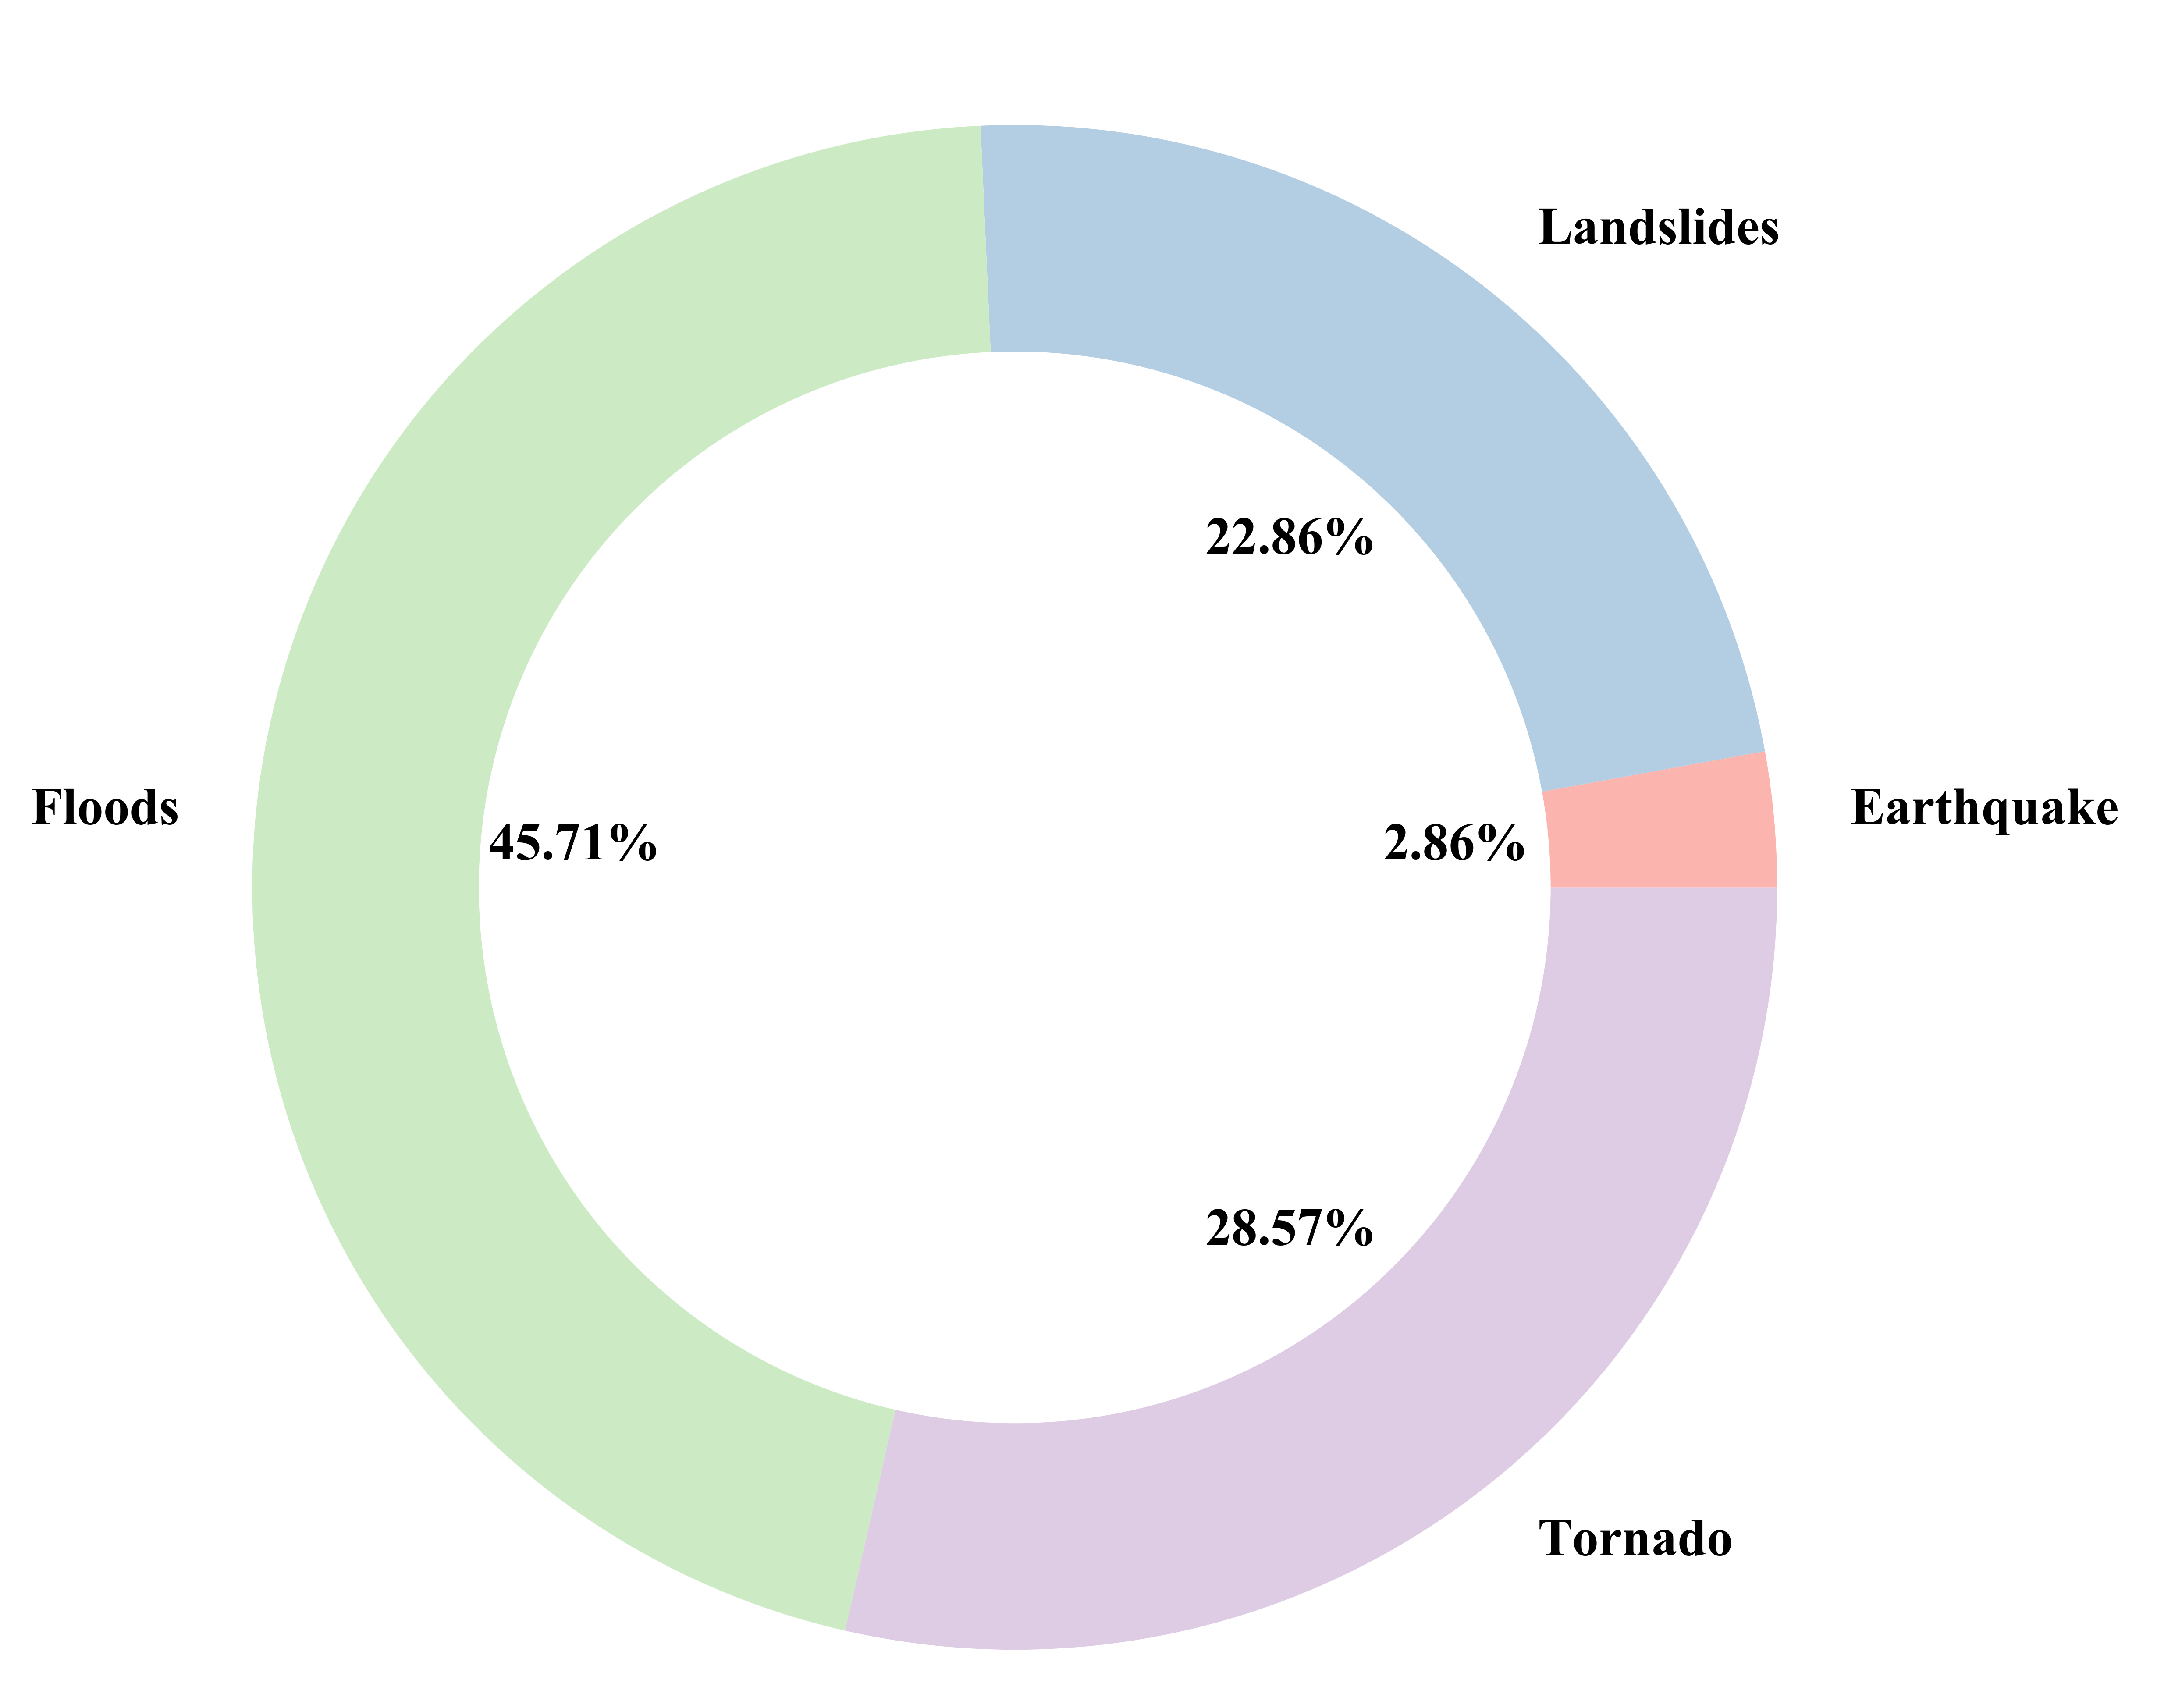
\includegraphics[scale=0.15]{foo.png}
\caption{Natural disasters occurred in Jakarta throughout 2018}
\end{center}
\end{figure}

\section{Motivation}

Based on the problem description above, it will be interesting to understand more of the nature of floods in Jakarta by utilizing the available public data. By using the data, the association between different types of variables can be drawn and an insight about why, when, or where the floods will occur in any given time can be predicted. Such an insight will be beneficial for the government, local authorities, the rescue teams, the medical teams, as well as all of the residents to have strategic measurements against upcoming floods.\\

\noindent
In this project, there are four main topics that will be discussed:
\begin{enumerate}
  \item The possible explanatory variable for the flood occurrence in Jakarta, in particular the rainfall rate, will be investigated. Then, the possible correlation between rainfall rate and the flood trends in Jakarta sub-districts throughout the year 2013 until 2017 will be studied. 
   \item The possible correlation between the rainfall rate with the amount of sub-district and people that will be affected by floods is also going to be studied. Based on possible correlation between these variables, a predictive modeling algorithm will be applied to predict future floods and their potential collateral damage.
   \item Based on the knowledge acquired from point number 1 and point number 2, the districts in Jakarta will be clustered into several segments to find out which districts that have potentially high or low risks of floods should a heavy rainfall pours down the city. 
   \item A variable that might be beneficial to mitigate floods, which is the amount of parks in each district, will be studied. To understand the correlation between the amount of parks and the severity of floods in each district, Pearson correlation method will be used.
\end{enumerate}

\section{Data Sources}
In order to conduct all of the steps in the motivation sections above, data from different sources will be used. 
\begin{enumerate}
\item The data regarding the rainfall rate will be fetched from the BPS website. The website contains public open datasets which are accessible to anybody. However, due to the limitations of the data, the rainfall rate that is going to be considered will be the rate in the span of 2013 until 2017.
\item The data regarding the amount of sub-districts as well as the number of people who are affected by floods will be fetched from Satu Data Indonesia, which is a website contains of several open datasets from the Indonesian government regarding national issues. Due to data limitations, the data that will be investigated is also going to be in the span of 2013-2017.
\item In order to get the name of all of the districts in Jakarta, the web-scraping approach from Wikipedia page will be applied.
\item To obtain the complete latitude and longitude coordinates for all of the districts in Jakarta, geopy library will be used.
\item In order to obtain the data regarding the amount of parks in any given districts, the Foursquare API will be used. Then, additional filtering of the data obtained from Foursquare API will be conducted if necessary. 
\end{enumerate}

\section{Data Features}
In this section, the features of the data sources that has been explained in the previous section will be explained.
\begin{enumerate}
\item \textbf{Data from the BPS:} There is one csv file from BPS website that contains the rainfall rate in any given month throughout the year 2009 until 2017. However in order to match the available data regarding the flood occurrences that will be explained in point number two, only the rainfall rate in the span of 2013 until 2017 will be considered.
\item  \textbf{Data from Satu Data Indonesia:} there are two different types of datasets that will be fetched from this website:

\begin{itemize}
\item Five csv files (2013 until 2017) in which each file contains an information about the flood occurrences in a given year (annual floods recapitulation).
\item More than 30 csv files that will be combined into a data frame in which each of the csv file contains an information about flood occurrences in a month from 2013 until 2016. The features that can be obtained from each file including the number of sub-districts affected by flood, the number of people affected by floods, days needed for each sub-district to recover from flood, and the number of people who are forced to relocate from their own house because of floods in any given month.
\end{itemize}
\item \textbf{Data from Wikipedia page:} there will be five different pages from Wikipedia that will be used to obtain the complete districts name of Jakarta. The url of each of the website is going to be listed in the Reference section.
\item \textbf{Data from Foursquare API:} with Foursquare API, a specific category of the place of interest can be defined in advance. In this project, a specific category, which is parks, will be used to obtain the list of the parks located in each district of Jakarta.
\end{enumerate}